\documentclass[11pt]{article}


\usepackage{graphicx}
\newcommand\be{\begin{equation}}
\newcommand\ee{\end{equation}}

\begin{document}
\title{Essential Equations}
\date{}
\author{Colt Bradley}
\maketitle

% Begin discussion of Newton’s laws of motion

\section{Newton’s Laws}
Newton`s first law says: ``Every body continues in its state
of rest, or of uniform motion in a right line, unless it is
compelled to change that state by forces impressed upon it."
Newton`s second law is

\begin{equation}
\vec F = m \vec a \label{Newton2}
\end{equation}

where $\vec F$ is the force on a particle of mass m, and
$\vec a$ is the particle`s acceleration. Newton`s second law (\ref{Newton2}) allows us to predict the future

Newton`s third law says:``for every action, there is an equal and opposite reaction"

\begin{figure}[ht]
\centering
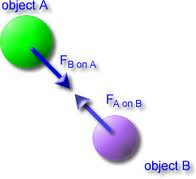
\includegraphics[scale=.5]{N3L.jpg}
\caption{Newton`s Third Law}
\end{figure}

% Begin discussion of Maxwell’s equations
\section{Maxwell’s Equations}
Maxwell’s equations include Gauss’s law, which reads

\begin{equation}
\oint \vec E \cdot d\vec a = \frac{Q}{\epsilon_0}
\end{equation}
in integral form.


Also included is Faraday's Law
\begin{equation}
\oint \vec E \cdot d\vec s = - \frac{d \Phi}{d t}
\end{equation}

And Ampere's Law (In differential form)
\be
\vec \nabla \times \vec B = \mu_0 \vec J + \mu_0 \epsilon_0 \frac{\partial \vec E}{\partial t}
\ee

And the final Maxwell equation, which seems on first glance trivial but in fact is essential.
\begin{equation}
\vec \nabla \cdot \vec B = 0
\end{equation}

\end{document}